%% Ashiv Dhondea
% 22 October 2015
% Perfect code
% 09/03/17: proper one. correct colors.
\documentclass{standalone}
\usepackage[dvipsnames]{xcolor}
\usepackage{tikz,amsmath}
\usepackage{tikz-3dplot}
\usetikzlibrary{shapes,calc,positioning,arrows}

\tikzset{measure length/.style={
              decoration={markings,
              mark connection node=a,
              mark =at position 0.5 with {
                 \node[transform shape,fill=white,scale=0.5,#1] (a) 
                        {\pgfmathparse{\pgfdecoratedpathlength/2.845274}%
                        \pgfmathprintnumber[fixed,precision=1]\pgfmathresult mm};},
             },
             postaction=decorate
       }
}

\begin{document}
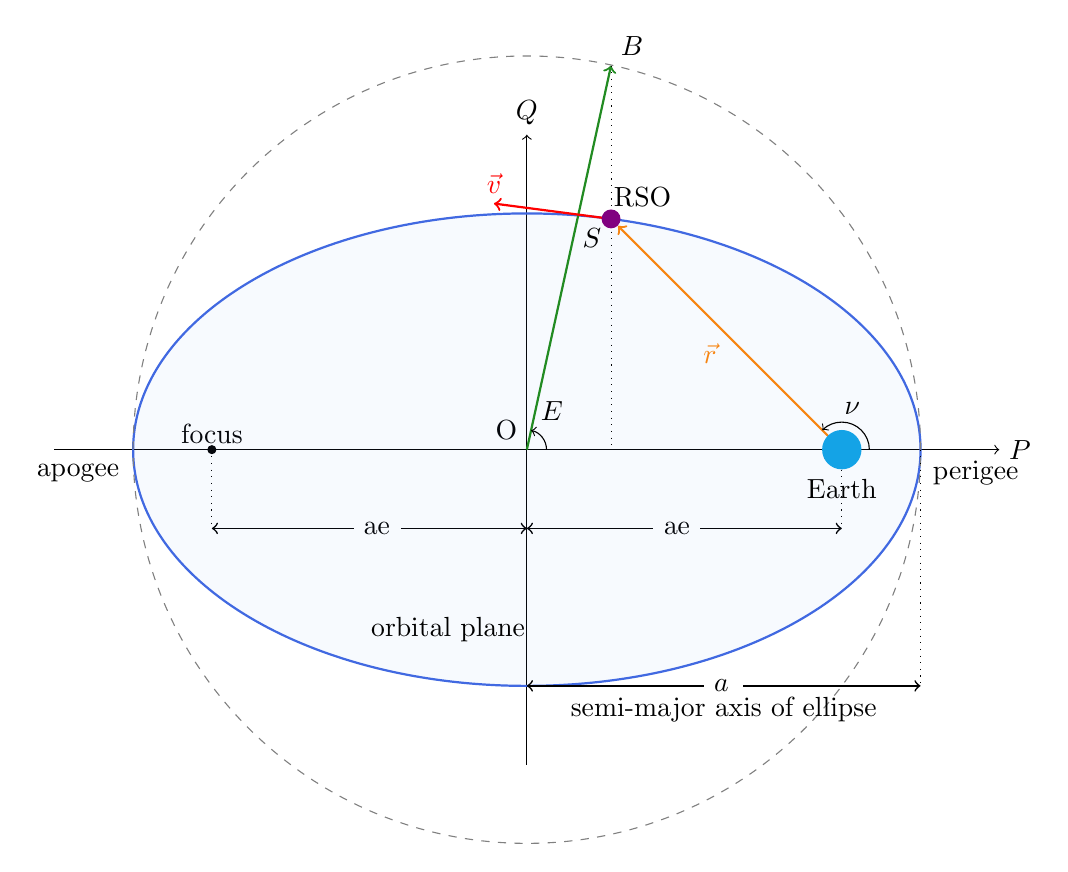
\begin{tikzpicture}
% Define the orbit
\pgfmathsetmacro{\t}{135} % True Anomaly value, deg
\pgfmathsetmacro{\e}{0.8} % Eccentricity
\pgfmathsetmacro{\a}{5} % Semi-Major Axis, cm
\pgfmathsetmacro{\v}{1.5} % Bogus velocity vector size, cm
 
% Compute some useful quantities
\pgfmathsetmacro{\b}{\a*sqrt(1-\e^2)} % Semi-Minor Axis, cm
\pgfmathsetmacro{\p}{\a*(1-\e^2)} % Semi-Latus Rectum, cm
\pgfmathsetmacro{\r}{ \p / (1 + \e*cos(\t))} % Radius, cm
\pgfmathsetmacro{\ff}{\e*\a}
\pgfmathsetmacro{\g}{atan(\r*\e*sin(\t) / \p)} % Flight path angle, deg
\pgfmathsetmacro{\adj}{\ff - \r*cos(180-\t)}

\draw	({\ff},0) node[anchor=east] {f};
\filldraw(-{\ff},0) circle (0.05);
\node[draw = none] at (-{\ff},0.2) {focus};
\draw[semithick,arrows=<-] (-{\ff},-1) -- ({-0.55*\ff},-1) node[anchor=west]{ae};
\draw[semithick,arrows=->] ({-0.40*\ff},-1) -- (0,-1);
\draw[dotted]({-\ff},0)--({-\ff},-1);

\draw[dotted]({\ff},0)--({\ff},-1);
\draw[semithick,arrows=<-] ({\ff},-1) -- ({0.55*\ff},-1) node[anchor=east]{ae};
\draw[semithick,arrows=->] ({0.40*\ff},-1) -- (0,-1);

\draw (0,0)node[anchor=south east]{O};
% Orbit reference frame, orbit, attracting body
\draw[->]({-\a-1},0) -- ({\a+1},0) node[anchor=west] {$P$};
\node[draw=none] at ({\a+1-0.3},-0.3) {perigee};
\node[draw=none] at ({-\a-1+0.3},-0.3) {apogee};
\draw[->](0, {-\b-1}) -- (0,{\b + 1}) node[anchor=south] {$Q$};
\draw[thick,RoyalBlue,fill =CornflowerBlue,fill opacity=0.05] (0,0) ellipse ({\a} and {\b});

\draw[dashed,Gray] (0,0) circle (\a);  % 2017

% h-direction
%\draw[->] (0.25,0) arc (0:340:0.25) node[anchor=north west] {$\hat{h}$};
%\draw[thick,green,->] (0,0)--({\ff - 0.99*\r*cos(\t)},{sqrt(\a^2-(\ff - 0.99*\r*cos(180-\t))^2)});
\draw[thick,ForestGreen,->](0,0)--({\ff - \r*cos(180-\t)},{sqrt(\a^2-(\ff - 0.99*\r*cos(180-\t))^2)});
\draw[dotted] ({\ff - \r*cos(180-\t)},{sqrt(\a^2-(\ff - 0.99*\r*cos(180-\t))^2)})--({\ff - \r*cos(180-\t)},0);
\draw	({\ff - \r*cos(180-\t)},{sqrt(\a^2-(\ff - 0.99*\r*cos(180-\t))^2)}) node[anchor=south west] {$B$};
\draw ({\ff - \r*cos(180-\t)},{\r*sin(180-\t)})node[anchor=north east]{$S$};
\node[draw = none] at ({\ff - \r*cos(180-\t) + 0.4} ,{\r*sin(180-\t) + 0.28}) {RSO};
\draw[->] (0.25,0) arc (0:{acos(\adj/\a))}:0.25) node[anchor=south west] {$E$};

% Dimensioning
\draw[semithick,arrows=<-] (0,-3) -- ({0.45*\a},-3)node[anchor=west]{$a$};
\node[draw = none]  at ({0.5*\a},-3.3){semi-major axis of ellipse};
\draw[semithick,arrows=->] ({0.55*\a},-3) -- ({\a},-3);
\draw[dotted]({\a},0)--({\a},-3);
\draw (-1,-2.) node[anchor=north] {orbital plane};

% Move center to attractive focus to make plotting easier
\begin{scope}[shift={({\ff},0)}]
% Position and Velocity vectors
\draw[thick, BurntOrange, ->](0,0) -- ({0.97*\r*cos(\t)}, {0.97*\r*sin(\t)});
\draw[BurntOrange] ({0.5*\r*cos(\t)}, {0.5*\r*sin(\t)}) node[anchor=north east]{$\vec{r}$};
\draw[thick,Red, ->]({\r*cos(\t)}, {\r*sin(\t)}) -- ({\r*cos(\t) + \v*cos(\t + 90 -\g)}, {\r*sin(\t) + \v*sin(\t + 90 -\g)}) node[anchor=south]{$\vec{v}$};
 
%\filldraw({\r*cos(\t)}, {\r*sin(\t)}) circle (0.05);
\path[fill=Purple]({\r*cos(\t)}, {\r*sin(\t)})circle(0.12);

% True Anomaly
\draw[->](0.35,0) arc (0:\t:0.35);
\draw ( {0.35*cos(\t/2)}, {0.35*sin(\t/2)} ) node[anchor=south] {$\nu$};

\path[fill=Cerulean](0,0)circle(0.25);
\node[draw = none] at (0,-0.5) {Earth};
\end{scope}
\end{tikzpicture}
\end{document}
